\documentclass[11pt,a4paper]{article}
\usepackage[utf8]{inputenc}
\usepackage[T1]{fontenc}
\usepackage{lmodern}
\usepackage[margin=25mm]{geometry}
\usepackage{amsmath,amssymb,mathtools,bm,array,xcolor,booktabs,longtable}
\usepackage{tikz,microtype,enumitem}
\usepackage[nolist]{acronym}
\usetikzlibrary{arrows.meta,positioning,fit}
\usepackage[colorlinks=true,linkcolor=blue!50!black,urlcolor=blue!50!black]{hyperref}
\newenvironment{example}[1]{\par\medskip\noindent\textbf{Worked example: #1.}\ }{\par\medskip}
\setlist[itemize]{noitemsep}
\numberwithin{equation}{section}
\setcounter{tocdepth}{1}

%%%%%%%%%%%%%%%%%%%%%%%%%%%%%%%%%%%%%%%%%%%%%%%%%%%%%%%%%%%%
% MIMO Communications - Common LaTeX Commands
%%%%%%%%%%%%%%%%%%%%%%%%%%%%%%%%%%%%%%%%%%%%%%%%%%%%%%%%%%%%
% Required packages:
% \usepackage{amsmath,amssymb,amsfonts}
% \usepackage{mathtools}
% \usepackage{bm}
% \usepackage{array}
% \usepackage{xcolor}
%
% Convention:
% - Scalars: italic
% - Vectors/matrices: bold lowercase/uppercase
% - Sets: calligraphic
% - Descriptive indices: \mathsf
% - Matrix transpose markers: \mathsf
% - Named mathematical operators: upright
%%%%%%%%%%%%%%%%%%%%%%%%%%%%%%%%%%%%%%%%%%%%%%%%%%%%%%%%%%%%


%%%%%%%%%%%%%%%%%%%%%%%%%%%%%%%%%%%%%%%%%%%%%%%%%%%%%%%%%%%%
% 1. REVIEW AND EDITING
%%%%%%%%%%%%%%%%%%%%%%%%%%%%%%%%%%%%%%%%%%%%%%%%%%%%%%%%%%%%

% Display old text [blue] and proposed text [red]
\newcommand{\Review}[2]{%
	{\color{blue}[#1]}{\color{red}[#2]}}

% Display corrected versions
\newcommand{\Fixed}[2]{%
	{\color{orange}[#1]}{\color{green}[#2]}}

% Show only the accepted version (first argument)
\newcommand{\Done}[2]{#1}

% Comments and notes
\newcommand{\Response}[1]{{\color{magenta}[#1]}}
\newcommand{\Note}[1]{{\color{blue}[#1]}}


%%%%%%%%%%%%%%%%%%%%%%%%%%%%%%%%%%%%%%%%%%%%%%%%%%%%%%%%%%%%
% 2. GENERAL UTILITIES
%%%%%%%%%%%%%%%%%%%%%%%%%%%%%%%%%%%%%%%%%%%%%%%%%%%%%%%%%%%%

% Fixed-width table columns with proper line breaks
\newcolumntype{C}[1]{>{\centering\arraybackslash}p{#1}}
\newcolumntype{R}[1]{>{\raggedleft\arraybackslash}p{#1}}
\newcolumntype{L}[1]{>{\raggedright\arraybackslash}p{#1}}

% Display literal LaTeX text
\newcommand{\ttplain}[1]{\texttt{\detokenize{#1}}}

% Underbraces for expressions in matrices/arrays
\newcommand{\undermat}[2]{%
	\makebox[0pt][l]{$%
		\smash{%
			\underbrace{%
				\phantom{\begin{matrix}#2\end{matrix}}%
			}_{\text{$#1$}}%
		}$}#2}

\newcommand{\coolunder}[2]{%
	\mathrlap{%
		\smash{%
			\underbrace{%
				\phantom{\begin{matrix}#2\end{matrix}}%
			}_{\mbox{$#1$}}%
		}%
	}#2}


%%%%%%%%%%%%%%%%%%%%%%%%%%%%%%%%%%%%%%%%%%%%%%%%%%%%%%%%%%%%
% 3. CROSS-REFERENCING
%%%%%%%%%%%%%%%%%%%%%%%%%%%%%%%%%%%%%%%%%%%%%%%%%%%%%%%%%%%%

\newcommand{\figref}[1]{Figure.~\ref{#1}}
\newcommand{\secref}[1]{Section~\ref{#1}}
\newcommand{\chapref}[1]{Chapter~\ref{#1}}
\newcommand{\theref}[1]{Theorem~\ref{#1}}
\newcommand{\appref}[1]{Appendix~\ref{#1}}
\newcommand{\tabref}[1]{Table~\ref{#1}}

% Define if not already provided by another package
\providecommand{\algref}[1]{}
\renewcommand{\algref}[1]{Algorithm~\ref{#1}}
% Additional packages for notation tables
\usepackage{longtable}
\usepackage{array}
%%%%%%%%%%%%%%%%%%%%%%%%%%%%%%%%%%%%%%%%%%%%%%%%%%%%%%%%%%%%
% 4. MATHEMATICAL OPERATORS AND DELIMITERS
%%%%%%%%%%%%%%%%%%%%%%%%%%%%%%%%%%%%%%%%%%%%%%%%%%%%%%%%%%%%

% Ceiling and floor (mathtools)
\DeclarePairedDelimiter{\ceil}{\lceil}{\rceil}
\DeclarePairedDelimiter{\floor}{\lfloor}{\rfloor}

% Optimization operators
\DeclareMathOperator*{\argmax}{arg\,max}
\DeclareMathOperator*{\argmin}{arg\,min}
\DeclareMathOperator*{\argfirst}{arg\,first}

% Angle/phase of complex quantity
% Overrides any existing \ang definition
\providecommand{\ang}[1]{}
\renewcommand{\ang}[1]{%
	\operatorname{angle}\left(#1\right)}

% Definition symbol
\newcommand{\define}{\triangleq}

% Delimiters (legacy commands)
\newcommand{\LeftP}{\left\lbrace}
\newcommand{\RightP}{\right\rbrace}
\newcommand{\LeftPD}{\left(}
\newcommand{\RightPD}{\right)}

% Additional delimiters
\newcommand{\Abs}[1]{\left|#1\right|}
\newcommand{\inner}[2]{%
	\left\langle #1,#2\right\rangle}


%%%%%%%%%%%%%%%%%%%%%%%%%%%%%%%%%%%%%%%%%%%%%%%%%%%%%%%%%%%%
% 5. SETS AND NUMBER FIELDS
%%%%%%%%%%%%%%%%%%%%%%%%%%%%%%%%%%%%%%%%%%%%%%%%%%%%%%%%%%%%

\newcommand{\compl}{\mathbb{C}}   % Complex field
\newcommand{\real}{\mathbb{R}}    % Real field
\newcommand{\intg}{\mathbb{Z}}    % Integers
\newcommand{\galois}{\mathbb{F}_2} % Binary finite field

% Calligraphic sets
\newcommand{\set}[1]{\mathcal{#1}}


%%%%%%%%%%%%%%%%%%%%%%%%%%%%%%%%%%%%%%%%%%%%%%%%%%%%%%%%%%%%
% 6. VECTORS AND MATRICES
%%%%%%%%%%%%%%%%%%%%%%%%%%%%%%%%%%%%%%%%%%%%%%%%%%%%%%%%%%%%

% Bold lowercase vectors and uppercase matrices
\newcommand{\ma}[1]{\bm{#1}}

% Element indexing
\newcommand{\IndexM}[3]{#1\left[#2,#3\right]}
\newcommand{\IndexV}[2]{#1\left[#2\right]}

% Norms
\newcommand{\Norm}[1]{\left\|#1\right\|}
\newcommand{\NormTwo}[1]{\left\|#1\right\|_2}
\newcommand{\frob}[1]{\left\|#1\right\|_{\mathsf{F}}}

% Matrix operations
\newcommand{\inv}[1]{{#1}^{-1}}
\newcommand{\pinv}[1]{{#1}^{+}}        % Pseudoinverse
\newcommand{\mT}[1]{{#1}^{\mathsf{T}}} % Transpose
\newcommand{\mH}[1]{{#1}^{\mathsf{H}}} % Hermitian transpose
\newcommand{\mC}[1]{{#1}^{*}}         % Complex conjugate

% Matrix properties and functions
\newcommand{\trace}[1]{%
	\operatorname{tr}\left(#1\right)}
\newcommand{\rank}[1]{%
	\operatorname{rank}\left(#1\right)}
\newcommand{\Cond}[1]{%
	\operatorname{cond}\left(#1\right)}
\newcommand{\Det}[1]{%
	\operatorname{det}\left(#1\right)}
\newcommand{\diag}[1]{%
	\operatorname{diag}\left(#1\right)}

% Alias for compatibility
\newcommand{\diagM}[1]{\diag{#1}}

% Vector subspaces
\newcommand{\Span}[1]{%
	\operatorname{span}\left(#1\right)}
\newcommand{\Null}[1]{%
	\operatorname{null}\left(#1\right)}
\newcommand{\Range}[1]{%
	\operatorname{range}\left(#1\right)}

% Vectorization and reshaping
\newcommand{\Vect}[1]{%
	\operatorname{vec}\left(#1\right)}
\newcommand{\unvec}[3]{%
	\operatorname{unvec}_{#2\times #3}\left(#1\right)}

% Matrix products
\newcommand{\elemProd}[2]{#1\odot #2}
\newcommand{\elemDiv}[2]{#1\oslash #2}
\newcommand{\kronProd}[2]{#1\otimes #2}


%%%%%%%%%%%%%%%%%%%%%%%%%%%%%%%%%%%%%%%%%%%%%%%%%%%%%%%%%%%%
% 7. PROBABILITY AND STATISTICS
%%%%%%%%%%%%%%%%%%%%%%%%%%%%%%%%%%%%%%%%%%%%%%%%%%%%%%%%%%%%

% Expectation and variance
\newcommand{\Ex}[1]{%
	\mathbb{E}\left[#1\right]}
\newcommand{\Var}[1]{%
	\operatorname{Var}\left[#1\right]}

% Covariance and correlation
\newcommand{\Cov}[2]{%
	\operatorname{Cov}\left(#1,#2\right)}
\newcommand{\Corr}[2]{%
	\operatorname{Corr}\left(#1,#2\right)}

% Probability of an event
\newcommand{\Prob}[1]{%
	\Pr\left(#1\right)}

% Mean-square error
\newcommand{\MSE}[1]{%
	\operatorname{MSE}\left(#1\right)}

% Distribution notation
\newcommand{\Normal}{\mathcal{N}}
\newcommand{\CNormal}{\mathcal{CN}}

% Complex signal operations
\newcommand{\RE}[1]{%
	\operatorname{Re}\left\{#1\right\}}
\newcommand{\IM}[1]{%
	\operatorname{Im}\left\{#1\right\}}


%%%%%%%%%%%%%%%%%%%%%%%%%%%%%%%%%%%%%%%%%%%%%%%%%%%%%%%%%%%%
% 8. SIGNAL PROCESSING OPERATIONS
%%%%%%%%%%%%%%%%%%%%%%%%%%%%%%%%%%%%%%%%%%%%%%%%%%%%%%%%%%%%

% Fourier transform
\newcommand{\FT}[1]{%
	\mathcal{F}\left\{#1\right\}}

% Circular convolution
\newcommand{\circConv}[2]{#1\circledast #2}

% Modulo reduction notation
\newcommand{\modulo}[2]{%
	\left\langle #1\right\rangle_{#2}}

% Sinc function
\newcommand{\Sinc}[1]{%
	\operatorname{sinc}\left(#1\right)}


%%%%%%%%%%%%%%%%%%%%%%%%%%%%%%%%%%%%%%%%%%%%%%%%%%%%%%%%%%%%
% 9. MIMO DIMENSIONS AND INDICES
%%%%%%%%%%%%%%%%%%%%%%%%%%%%%%%%%%%%%%%%%%%%%%%%%%%%%%%%%%%%

% Subscripts t/r: transmit/receive interfaces
% Superscripts rf/a: RF-chain/antenna-element interfaces
% No superscript: effective digital signal ports
% S: number of data streams
%
% Descriptive indices are upright (\mathsf).
% Running mathematical indices are italic..

% Digital signal ports
\newcommand{\NT}{N_{\mathsf{t}}}
\newcommand{\NR}{N_{\mathsf{r}}}
\newcommand{\nT}{n_{\mathsf{t}}}
\newcommand{\nR}{n_{\mathsf{r}}}

% Data streams
\newcommand{\NS}{S}
\newcommand{\nS}{s}

% RF chains
\newcommand{\NTrf}{N_{\mathsf{t}}^{\mathsf{rf}}}
\newcommand{\NRrf}{N_{\mathsf{r}}^{\mathsf{rf}}}
\newcommand{\nTrf}{n_{\mathsf{t}}^{\mathsf{rf}}}
\newcommand{\nRrf}{n_{\mathsf{r}}^{\mathsf{rf}}}

% Physical antenna elements
\newcommand{\NTa}{N_{\mathsf{t}}^{\mathsf{a}}}
\newcommand{\NRa}{N_{\mathsf{r}}^{\mathsf{a}}}
\newcommand{\nTa}{n_{\mathsf{t}}^{\mathsf{a}}}
\newcommand{\nRa}{n_{\mathsf{r}}^{\mathsf{a}}}


%%%%%%%%%%%%%%%%%%%%%%%%%%%%%%%%%%%%%%%%%%%%%%%%%%%%%%%%%%%%
% 10. MIMO PRECODING AND COMBINING MATRICES
%%%%%%%%%%%%%%%%%%%%%%%%%%%%%%%%%%%%%%%%%%%%%%%%%%%%%%%%%%%%

% Digital precoding and combining
\newcommand{\FD}{\ma{F}_{\mathsf{D}}}
\newcommand{\WD}{\ma{W}_{\mathsf{D}}}

% Analog precoding and combining
\newcommand{\FA}{\ma{F}_{\mathsf{A}}}
\newcommand{\WA}{\ma{W}_{\mathsf{A}}}


% MIMO channel representations

\newcommand{\Ha}{\ma{H}_{\mathsf{a}}}
% Antenna-level channel (physical antenna elements)

\newcommand{\Hrf}{\ma{H}_{\mathsf{rf}}}
% Effective channel after analog TX/RX processing


% H_a: Physical antenna-to-antenna channel
% H_rf: Effective channel between RF-chain interfaces
% H: Effective channel between digital signal ports
% H_s: Effective channel between data streams
%
% H_rf = W_A^H H_a F_A
% H    = W_D^H H_rf F_D
% H_s  = W^H H F


\newcommand{\Hs}{\ma{H}_{\mathsf{s}}}
% Effective stream-level channel after digital
% precoding and combining

% Diversity and multiplexing performance
\providecommand{\odiv}{o_{\mathsf{div}}}   % Diversity order
\providecommand{\gmux}{g_{\mathsf{mux}}}   % Multiplexing gain


%%%%%%%%%%%%%%%%%%%%%%%%%%%%%%%%%%%%%%%%%%%%%%%%%%%%%%%%%%%%
% 11. SIGNAL ENERGY AND NOISE
%%%%%%%%%%%%%%%%%%%%%%%%%%%%%%%%%%%%%%%%%%%%%%%%%%%%%%%%%%%%

\newcommand{\Es}{E_{\mathsf{s}}} % Energy per symbol
\newcommand{\Ed}{E_{\mathsf{d}}} % Total energy

\newcommand{\Eb}{E_{\mathsf{b}}} % Energy per bit

% Noise power spectral density parameter
\newcommand{\Nzero}{N_{0}}

\newcommand{\Ptx}{P_{\mathsf{t}}}
\newcommand{\Prx}{P_{\mathsf{r}}}


%%%%%%%%%%%%%%%%%%%%%%%%%%%%%%%%%%%%%%%%%%%%%%%%%%%%%%%%%%%%
% 12. COMMUNICATION METRICS AND ALGORITHMS
%%%%%%%%%%%%%%%%%%%%%%%%%%%%%%%%%%%%%%%%%%%%%%%%%%%%%%%%%%%%

\newcommand{\SNR}{\mathsf{SNR}}
\newcommand{\SINR}{\mathsf{SINR}}
\newcommand{\CSI}{\mathsf{CSI}}

% Combining and precoding
\newcommand{\MRT}{\mathsf{MRT}}
\newcommand{\MRC}{\mathsf{MRC}}
\newcommand{\ZF}{\mathsf{ZF}}
\newcommand{\LMMSE}{\mathsf{LMMSE}}

% Additional commonly used methods
\newcommand{\LS}{\mathsf{LS}}
\newcommand{\MMSE}{\mathsf{MMSE}}
\newcommand{\ML}{\mathsf{ML}}
\newcommand{\MAP}{\mathsf{MAP}}
\newcommand{\RZF}{\mathsf{RZF}}





%%%%%%%%%%%%%%%%%%%%%%%%%%%%%%%%%%%%%%%%%%%%%%%%%%%%%%%%%%%%
% End of common notation
%%%%%%%%%%%%%%%%%%%%%%%%%%%%%%%%%%%%%%%%%%%%%%%%%%%%%%%%%%%%
\providecommand{\RH}{R_{\ma H}}
\title{MIMO Communications\\Lecture 04: Multiuser MIMO Fundamentals}
\author{Ahmad Nimr}
\date{Winter Semester 2026/27}
\begin{document}
\begin{acronym}
	\acro{p2p}[P2P]{point-to-point}
	\acro{mimo}[MIMO]{multiple-input multiple-output}
	\acro{siso}[SISO]{single-input single-output}
	\acro{simo}[SIMO]{single-input multiple-output}
	\acro{miso}[MISO]{multiple-input single-output}
	\acro{mrc}[MRC]{maximum ratio combining}
	\acro{mrt}[MRT]{maximum ratio transmission}
	\acro{zf}[ZF]{zero forcing}
	\acro{lmmse}[LMMSE]{linear minimum mean-square error}
	\acro{mmse}[MMSE]{minimum mean-square error}
	\acro{svd}[SVD]{singular value decomposition}
	\acro{evd}[EVD]{eigenvalue decomposition}
	\acro{snr}[SNR]{signal-to-noise ratio}
	\acro{sinr}[SINR]{signal-to-interference-plus-noise ratio}
	\acro{csi}[CSI]{channel state information}
	\acro{csir}[CSIR]{channel state information at the receiver}
	\acro{csit}[CSIT]{channel state information at the transmitter}
	\acro{rf}[RF]{radio frequency}
	\acro{qpsk}[QPSK]{quadrature phase-shift keying}
	\acro{awgn}[AWGN]{additive white Gaussian noise}
	\acro{psd}[PSD]{power spectral density}
	\acro{map}[MAP]{maximum a posteriori}
	\acro{mse}[MSE]{mean squared error}
	\acro{ls}[LS]{least squares}
	\acro{ml}[ML]{maximum likelihood }
	\acro{bpsk}[BPSK]{binary phase-shift keying}
	\acro{iid}[IID]{independent and identically distributed}
	\acro{los}[LOS]{line of sight}
	\acro{ostbc}[OSTBC]{orthogonal space-time block code}
	\acro{stbc}[STBC]{space-time block code}
	\acro{dmt}[DMT]{diversity--multiplexing tradeoff}
	\acro{pdf}[PDF]{probability density function}
	\acro{mumimo}[MU-MIMO]{multiuser multiple-input multiple-output}
	\acro{ul}[UL]{uplink}
	\acro{dl}[DL]{downlink}
	\acro{fdma}[FDMA]{frequency-division multiple access}
	\acro{tdma}[TDMA]{time-division multiple access}
	\acro{sdma}[SDMA]{space-division multiple access}
	\acro{bs}[BS]{base station}
	\acro{mac}[MAC]{multiple-access channel}
	\acro{bc}[BC]{broadcast channel}
	\acro{rzf}[RZF]{regularized zero forcing}
	\acro{sic}[SIC]{successive interference cancellation}
	\acro{dpc}[DPC]{dirty-paper coding}
	\acro{dof}[DoF]{degrees of freedom}
	\acro{tdd}[TDD]{time-division duplex}
	\acro{fdd}[FDD]{frequency-division duplex}
	\acro{ap}[AP]{access point}
	\acro{cpu}[CPU]{central processing unit}
	\acro{comp}[CoMP]{coordinated multipoint}
	\acro{cscg}[CSCG]{circularly symmetric complex Gaussian}
	\acro{mu}[MU]{multi-user}
	\acro{se}[SE]{spectral efficiency}
\end{acronym}

\acresetall
\maketitle
\begin{abstract}
Multiuser MIMO distributes spatial streams among independently operating terminals. This lecture develops uplink and downlink signal models, separates desired signals from interuser interference, and derives maximum-ratio, zero-forcing, and regularized linear processing. Energy normalization and the location of joint processing distinguish the two directions. Achievable rates and a two-user example connect channel geometry to receiver noise enhancement and transmit-energy penalties. Large-array statistics and distributed deployment are deferred to Lecture~05.
\end{abstract}
\acresetall
\tableofcontents
\newpage


\section{Multiple access and the transition to multiuser MIMO}

\subsection{Learning objectives and connection to previous lectures}
Lectures~01--03 established the digital channel model, linear stream processing, and statistical performance of a \ac{p2p} \ac{mimo} link. In \ac{mumimo}, independent user terminals share the spatial resources of a common \ac{bs}. The central question is whether the users have sufficiently distinct channel responses across the BS antenna ports to support simultaneous communication. These responses are represented by user channel vectors, whose entries describe the complex channel coefficients between each user and the BS antenna ports. Antenna count, channel rank, channel gain, and conditioning remain the relevant tools; their interpretation now concerns different users rather than streams of one cooperating terminal.

After this lecture, students should be able to formulate dimensionally consistent \ac{ul} and \ac{dl} models and distinguish independent user energy constraints from a common BS energy constraint. They should also be able to derive linear combining and precoding directions, calculate user \ac{sinr} and Gaussian achievable rates, and explain how channel geometry limits user separation. The development assumes a narrowband channel fixed over the considered processing interval, synchronized signals, and perfect channel knowledge where required. Statistical averaging uses the models of Lecture~03.

\subsection{Orthogonal resources and spatial sharing}
Multiple access assigns communication resources to different users. \Ac{fdma} separates users in frequency, whereas \ac{tdma} separates them in time. Ideal orthogonal allocation removes mutual interference within the allocated resources, but each user receives only a fraction of the total bandwidth or time. \Ac{sdma} instead exploits differences between user channel responses across the antenna ports to serve users on the same time-frequency resource. Unlike FDMA and TDMA, spatial separation depends on the channel and may be imperfect. SDMA can be combined with frequency and time allocation: a scheduler selects a group of users, and spatial processing enables simultaneous communication while managing interuser interference.

\begin{center}
	\begin{tabular}{lll}
		\toprule
		Method & Separating resource & Main processing requirement\\
		\midrule
		\acs{fdma} & Frequency bands & Filtering and frequency allocation\\
		\acs{tdma} & Time intervals & Timing and time allocation\\
		\acs{sdma} & Spatial channel differences & Channel knowledge and spatial processing\\
		\bottomrule
	\end{tabular}
\end{center}
Orthogonal allocation gives each user only a fraction of the system resource. Comparisons with simultaneous spatial transmission must use the same resource and energy normalization; the rate accounting is revisited in Section~\ref{sec:rates}.

\subsection{Cooperation distinguishes P2P and multiuser operation}
In P2P spatial multiplexing, several streams belong to one communication link. Multiple access assigns streams to different users, potentially with independent constraints and decoding. In a P2P link, all receive observations are available to a common receiver, allowing joint spatial processing and potentially joint decoding. In the uplink, the BS can similarly process observations from several independent transmitters, whereas in the downlink, the BS controls all transmitted streams but the user terminals generally decode their messages independently.

This distinction limits the direct application of P2P processing methods. For example, singular-value decomposition of an aggregate downlink channel generally requires a receiver-side singular-vector rotation that mixes observations from different users. Such a rotation cannot be implemented independently at each terminal without exchanging received signals, even though the aggregate channel can be represented by a matrix.

\begin{figure}[ht]
	\centering
	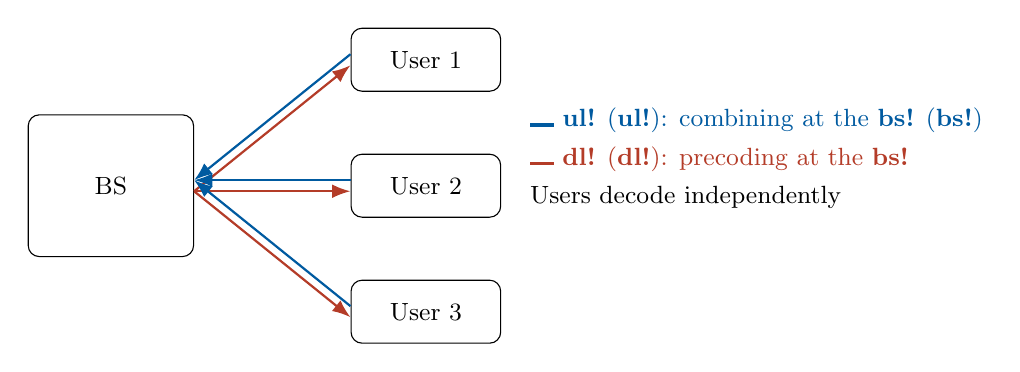
\begin{tikzpicture}[>=Latex,font=\small]
		% colors
		\definecolor{ulcolor}{RGB}{0,90,160}
		\definecolor{dlcolor}{RGB}{180,60,40}
		
		% nodes
		\node[draw,rounded corners,minimum width=21mm,minimum height=18mm] (bs) at (0,0) {BS};
		
		\foreach \u/\y in {1/1.6,2/0,3/-1.6}{
			\node[draw,rounded corners,minimum width=19mm,minimum height=8mm] (u\u) at (4,\y) {User $\u$};
			
			% UL arrow: user -> BS
			\draw[->,ulcolor,thick]
			([yshift=2.0pt]u\u.west) -- ([yshift=2.0pt]bs.east);
			
			% DL arrow: BS -> user
			\draw[->,dlcolor,thick]
			([yshift=-2.0pt]bs.east) -- ([yshift=-2.0pt]u\u.west);
		}
		
		% legend / explanation
		\node[align=left,anchor=west] at (5.2,0.35) {%
			\textcolor{ulcolor}{\rule{3mm}{1.2pt}\ \ac{ul}: combining at the \ac{bs}}\\[1mm]
			\textcolor{dlcolor}{\rule{3mm}{1.2pt}\ \ac{dl}: precoding at the \ac{bs}}\\[1mm]
			Users decode independently};
	\end{tikzpicture}
	\caption{\ac{sdma} conceptual configuration. The \ac{bs} communicates with multiple users over the same time-frequency resource. In the \ac{ul}, user signals are combined at the \ac{bs}; in the \ac{dl}, the \ac{bs} applies precoding before transmission.}
	\label{fig:conceptual-sdma}
\end{figure}

\figref{fig:conceptual-sdma} illustrates the common communication configuration for \ac{sdma}; the precise \ac{ul} and \ac{dl} channel conventions are introduced in the next section.
%
The \ac{ul} is a \ac{mac}, while the \ac{dl} is a \ac{bc}. These terms describe the communication configuration rather than a particular processing algorithm. Beyond linear processing, joint decoding and \ac{sic} can exploit the structure of multiple user signals at the receiver. In the downlink, \ac{dpc} is a nonlinear transmitter-side coding technique that exploits interference known in advance during encoding, rather than explicitly canceling it through linear precoding. These techniques provide information-theoretic performance benchmarks but are not developed in this lecture.


\section{Multiuser MIMO system models}
\label{sec:models}

\subsection{System configuration and notation}
A \ac{bs} jointly receives signals from multiple users in the \ac{ul} and jointly generates their transmit signals in the \ac{dl}. Initially, $U$ users with one effective digital antenna port and one stream each are considered. The BS has $\NR$ receive ports in the UL and $\NT$ transmit ports in the DL. Multi-antenna users are considered at the end of this section.

\begin{table}[ht]
	\centering
	\small
	\caption{Dimensions of the main quantities for single-port users.}
	\label{tab:mu-dimensions}
	\begin{tabular}{lll}
		\toprule
		Quantity & Uplink & Downlink\\
		\midrule
		BS digital ports & $\NR$ receive ports & $\NT$ transmit ports\\
		User channel $\ma h_u$ & $\ma h_u^{\mathsf{UL}}\in\compl^{\NR\times1}$ & $\ma h_u^{\mathsf{DL}}\in\compl^{\NT\times1}$\\
		Channel matrix $\ma H$ & $\ma H_{\mathsf{UL}}\in\compl^{\NR\times U}$ & $\ma H_{\mathsf{DL}}\in\compl^{\NT\times U}$\\
		BS processing & $\ma W\in\compl^{\NR\times U}$ & $\ma F\in\compl^{\NT\times U}$\\
		Noise covariance & $\sigma_v^2\ma I_{\NR}$ & $\sigma_u^2$ at user $u$\\
		\bottomrule
	\end{tabular}
\end{table}

\tabref{tab:mu-dimensions} summarizes the dimensions. The superscripts $\mathsf{UL}$ and $\mathsf{DL}$ distinguish the channel directions; $\ma h_u$ and $\ma H$ are used for either direction when no ambiguity arises. In both cases, the user channel vectors form the columns of $\ma H$. The UL mapping is $\ma H_{\mathsf{UL}}$, whereas the DL mapping is $\mT{\ma H}_{\mathsf{DL}}$. No equality between the two channel matrices is assumed.

\subsection{Uplink multiple-access channel}
In the UL, user $u$ transmits a scalar symbol $x_u$ over $\ma h_u=\ma h_u^{\mathsf{UL}}$. The received BS signal is
\begin{equation}
	\boxed{\ma y=\sum_{u=1}^{U}\ma h_u x_u+\ma v=\ma H\ma x+\ma v},\qquad
	\ma H=[\ma h_1,\ldots,\ma h_U]\in\compl^{\NR\times U},
	\label{eq:ulmodel}
\end{equation}
where $\ma x=[x_1,\ldots,x_U]^{\mathsf T}$. Independent zero-mean user symbols are assumed, with individual transmitted symbol energies
\begin{equation}
	\Ex{|x_u|^2}=E_u,\qquad
	\ma R_x=\Ex{\ma x\mH{\ma x}}=\diag{E_1,\ldots,E_U}.
	\label{eq:ulenergy}
\end{equation}
Each user has its own energy budget $E_u$ per complex channel use; no common uplink sum-energy constraint is imposed. The receiver noise is assumed independent of the symbols and \ac{cscg}, $\ma v\sim\mathcal{CN}(\ma 0,\ma R_v)$, with $\ma R_v=\ma C_v=\sigma_v^2\ma I_{\NR}$ unless stated otherwise. For a fixed channel, the received second moment is
\begin{equation}
	\ma R_y=\ma H\ma R_x\mH{\ma H}+\ma R_v.
	\label{eq:ulcov}
\end{equation}
The user channels are assumed known at the BS for coherent combining. The individual transmitters need not know the instantaneous channels of other users. \eqref{eq:ulmodel} resembles a P2P MIMO channel, but its inputs originate from independent terminals with separate energy constraints.

\subsection{Downlink broadcast channel}
In the DL, the BS precodes independent symbols for the users. With $\ma h_u=\ma h_u^{\mathsf{DL}}$, the transmitted and received signals are
\begin{align}
	\ma x&=\sum_{u=1}^{U}\ma f_u d_u=\ma F\ma d,
	&\ma F&=[\ma f_1,\ldots,\ma f_U]\in\compl^{\NT\times U},\\
	y_u&=\mT{\ma h}_u\ma F\ma d+v_u,
	&\ma y&=\mT{\ma H}\ma F\ma d+\ma v.
	\label{eq:dlmodel}
\end{align}
Thus, $\ma H=[\ma h_1,\ldots,\ma h_U]$ contains the user channel columns, while $\mT{\ma H}\in\compl^{U\times\NT}$ is the DL channel mapping. With this convention, the maximum-ratio transmit direction is $\ma h_u^*$.

All DL streams share the BS energy budget $\Ed$. Following Lecture~02, independent zero-mean symbols and the normalized precoder satisfy
\begin{equation}
	\ma R_d=\Ex{\ma d\mH{\ma d}}=\Ed\ma I_U,
	\qquad \frob{\ma F}^2\leq1.
	\label{eq:dlconstraint}
\end{equation}
Consequently,
\begin{equation}
	\ma R_x=\Ed\ma F\mH{\ma F},\qquad
	\Ex{\NormTwo{\ma x}^2}=\Ed\frob{\ma F}^2\leq\Ed.
	\label{eq:dlenergy}
\end{equation}
For unit-norm beam directions $\ma b_u$, the columns may be written as
\begin{equation}
	\ma f_u=\sqrt{\alpha_u}\,\ma b_u,\qquad
	\NormTwo{\ma b_u}=1,\quad \alpha_u\geq0,\quad
	\sum_{u=1}^{U}\alpha_u\leq1.
	\label{eq:beamenergy}
\end{equation}
Thus, $\alpha_u$ is the fraction of the BS energy budget assigned to user $u$, corresponding to $\Ed\alpha_u$ per channel use. Energy allocation is included in $\ma F$ and is not applied again through $\ma R_d$.

The noise $v_u$ is assumed \ac{cscg}, independent across users, with variance $\sigma_u^2$. Channel-dependent precoding requires suitable \ac{csit}; coherent detection at user $u$ requires its effective desired channel gain. CSI acquisition is discussed in Lecture~05.

\subsection{Uplink and downlink comparison}
In the UL, combining is performed after noise and interference are received. Rescaling a combining vector by a nonzero scalar does not change its \ac{sinr}. In the DL, precoding is performed before transmission, and beam scaling changes the allocated transmit energy. Thus, channel inversion can cause noise enhancement in UL combining and a transmit-energy penalty in DL precoding. The distinction is important for the linear methods considered next.

\subsection{Duplexing and channel reciprocity}
In \ac{tdd}, UL and DL use the same frequency band at different times; in \ac{fdd}, they use separate frequency bands. TDD allows UL measurements to support DL channel estimation when the channel remains sufficiently stable. In FDD, the frequency difference generally prevents direct reuse of instantaneous UL channel coefficients, so DL measurements and feedback are commonly required.

For the same frequency and matching physical antenna ports, reciprocal propagation gives $\ma H_{\mathsf{DL}}=\ma H_{\mathsf{UL}}$ under the adopted transpose convention. However, $\NT$ and $\NR$ may differ because different digital ports or RF chains are used in the two directions. In that case, this equality cannot be applied to the complete effective channel matrices; reciprocity can only be related through the corresponding common physical ports and their processing mappings. Moreover, transmit and receive hardware responses generally differ. Appropriate calibration is therefore required before UL measurements can be used to infer the effective DL digital channel. No reciprocity assumption is required for the signal models above.

\subsection{Extension to multi-antenna users}
The models can be extended to users with $N_{\mathsf t,u}$ transmit ports and $N_{\mathsf r,u}$ receive ports. In the UL, user $u$ sends $S_u\leq N_{\mathsf t,u}$ streams through $\ma F_u\in\compl^{N_{\mathsf t,u}\times S_u}$. With $\ma H_u^{\mathsf{UL}}\in\compl^{\NR\times N_{\mathsf t,u}}$, the received signal becomes
\begin{equation}
	\ma y=\sum_{u=1}^{U}\ma H_u^{\mathsf{UL}}\ma F_u\ma d_u+\ma v,
	\qquad \ma d_u\in\compl^{S_u\times1}.
	\label{eq:ulmultiuser}
\end{equation}
The total user energy constraint applies across all its ports and streams:
\begin{equation}
	\Ex{\NormTwo{\ma x_u}^2}
	=\trace{\ma F_u\ma R_{d_u}\mH{\ma F_u}}\leq E_u,
	\qquad \ma x_u=\ma F_u\ma d_u,
	\label{eq:ulmultiuserenergy}
\end{equation}
where $\ma R_{d_u}=\Ex{\ma d_u\mH{\ma d_u}}$.

In the DL, user $u$ receives through $\ma H_u^{\mathsf{DL}}\in\compl^{N_{\mathsf r,u}\times\NT}$. For $\ma F_j\in\compl^{\NT\times S_j}$, its received vector is
\begin{equation}
	\ma y_u=\ma H_u^{\mathsf{DL}}\sum_{j=1}^{U}\ma F_j\ma d_j+\ma v_u.
	\label{eq:dlmultiuser}
\end{equation}
A local combiner $\ma W_u\in\compl^{N_{\mathsf r,u}\times S_u}$ may be applied. The BS energy constraint remains shared among all DL streams. The following sections focus on single-port users, for whom the main MU-MIMO principles can be developed without additional block-matrix notation.


\section{Linear combining and precoding}
\label{sec:processing}

\subsection{Effective channels and user interference}
In the UL, the received signal is processed by a combining matrix $\ma W=[\ma w_1,\ldots,\ma w_U]\in\compl^{\NR\times U}$, giving $\widehat{\ma x}=\mH{\ma W}\ma y$. In the DL, the data symbols are processed by the precoding matrix $\ma F=[\ma f_1,\ldots,\ma f_U]\in\compl^{\NT\times U}$. The corresponding effective channels are
\begin{equation*}
	\ma H_{\mathsf s}^{\mathsf{UL}}=\mH{\ma W}\ma H,
	\qquad
	\ma H_{\mathsf s}^{\mathsf{DL}}=\mT{\ma H}\ma F,
\end{equation*}
both in $\compl^{U\times U}$. The diagonal entries represent desired user channels, while the off-diagonal entries represent interuser interference. Since the users decode their messages independently, the interfering signals are treated as noise in the following linear processing methods.

\subsection{General signal decomposition and SINR}
The combined UL signal for user $u$ is
\begin{equation*}
	\widehat x_u=
	\underbrace{\mH{\ma w}_u\ma h_u x_u}_{\text{desired signal}}
	+\underbrace{\sum_{j\ne u}\mH{\ma w}_u\ma h_jx_j}_{\text{interuser interference}}
	+\underbrace{\mH{\ma w}_u\ma v}_{\text{noise}}.
\end{equation*}
For independent user symbols with energies $E_u$ and CSCG noise with covariance $\ma R_v$, the instantaneous \ac{sinr} is
\begin{equation}
	\boxed{
		\gamma_u^{\mathsf{UL}}=
		\frac{E_u|\mH{\ma w}_u\ma h_u|^2}
		{\displaystyle\sum_{j\ne u}E_j|\mH{\ma w}_u\ma h_j|^2+
			\mH{\ma w_u}\ma R_v\ma w_u}.
	}
	\label{eq:ulsinr}
\end{equation}
For spatially white noise, the last term becomes $\sigma_v^2\NormTwo{\ma w_u}^2$. Scaling $\ma w_u$ by any nonzero complex scalar leaves the SINR unchanged.

In the DL, the received signal at user $u$ is
\begin{equation*}
	y_u=
	\underbrace{\mT{\ma h}_u\ma f_u d_u}_{\text{desired signal}}
	+\underbrace{\sum_{j\ne u}\mT{\ma h}_u\ma f_jd_j}_{\text{interuser interference}}
	+\underbrace{v_u}_{\text{noise}},
\end{equation*}
with instantaneous SINR
\begin{equation}
	\boxed{
		\gamma_u^{\mathsf{DL}}=
		\frac{\Ed|\mT{\ma h}_u\ma f_u|^2}
		{\displaystyle\Ed\sum_{j\ne u}|\mT{\ma h}_u\ma f_j|^2+\sigma_u^2}.
	}
	\label{eq:dlsinr}
\end{equation}
Unlike UL combining, scaling a DL precoding column changes its transmitted energy and the interference received by other users. The precoder must therefore satisfy the common BS energy constraint.

\subsection{Maximum-ratio combining and transmission}
For spatially white noise, the Cauchy--Schwarz inequality gives
\begin{equation*}
	\frac{|\mH{\ma w}_u\ma h_u|^2}{\NormTwo{\ma w_u}^2}
	\leq\NormTwo{\ma h_u}^2.
\end{equation*}
Equality is attained for $\ma w_u\propto\ma h_u$. The \ac{mrc} combiner $\ma w_u=\ma h_u$ therefore maximizes the desired signal-to-noise ratio, but not generally the SINR in the presence of other users. Substitution into \eqref{eq:ulsinr} gives
\begin{equation}
	\gamma_u^{\mathsf{UL},\MRC}
	=\frac{E_u\NormTwo{\ma h_u}^4}
	{\displaystyle\sum_{j\ne u}E_j|\mH{\ma h}_u\ma h_j|^2+
		\sigma_v^2\NormTwo{\ma h_u}^2}.
	\label{eq:mrc}
\end{equation}

In the DL, \ac{mrt} maximizes the desired received energy for a fixed transmit-beam energy $\alpha_u \Ed$. Under the transpose-based channel convention, the corresponding beam direction and precoder are
\begin{equation*}
	\ma b_u=\frac{\ma h_u^*}{\NormTwo{\ma h_u}},
	\qquad
	\ma f_u=\sqrt{\alpha_u}\,\ma b_u,
\end{equation*}
where $\alpha_u\geq0$ and $\sum_u \alpha_u\leq1$. The desired received energy is $\alpha_u\Ed\NormTwo{\ma h_u}^2$, while beam $j$ contributes interference energy
\begin{equation*}
	\alpha_j\Ed\frac{|\mT{\ma h}_u\ma h_j^*|^2}
	{\NormTwo{\ma h_j}^2}.
\end{equation*}
Maximum-ratio processing requires no channel inversion, but does not explicitly suppress interuser interference. Orthogonal user channels eliminate this interference, whereas aligned channels cannot be separated by maximum-ratio processing.

\subsection{Uplink zero forcing}
For a full-column-rank channel with $\rank{\ma H}=U\leq\NR$, the \ac{zf} combiner is
\begin{equation}
	\boxed{
		\ma W_{\ZF}=\ma H\inv{(\mH{\ma H}\ma H)},
		\qquad
		\mH{\ma W}_{\ZF}\ma H=\ma I_U.
	}
	\label{eq:ulzf}
\end{equation}
The combined signal becomes $\widehat{\ma x}=\ma x+\mH{\ma W}_{\ZF}\ma v$. For spatially white noise, the output noise covariance and user SINR are
\begin{equation}
	\ma R_{v_{\mathsf c}}
	=\sigma_v^2\inv{(\mH{\ma H}\ma H)},
	\qquad
	\boxed{
		\gamma_u^{\mathsf{UL},\ZF}
		=\frac{E_u}
		{\sigma_v^2[\inv{(\mH{\ma H}\ma H)}]_{uu}}.
	}
	\label{eq:ulzfsinr}
\end{equation}
ZF eliminates interuser interference but may amplify the received noise when the channel is poorly conditioned. If the full-column-rank condition is not satisfied, a pseudoinverse cannot recover all independent user symbols without residual interference.

\subsection{Downlink zero forcing and normalization}
For $\rank{\ma H}=U\leq\NT$, the unnormalized DL ZF matrix is
\begin{equation}
	\ma B=\ma H^*\inv{(\mT{\ma H}\ma H^*)},
	\qquad
	\mT{\ma H}\ma B=\ma I_U.
	\label{eq:dlzfdirection}
\end{equation}
The precoder must additionally satisfy the common BS energy constraint. With global normalization,
\begin{align}
	\ma F_{\ZF}&=\xi\ma B,
	&
	\xi&=\frac{1}{\frob{\ma B}}
	=\left(\trace{\inv{(\mT{\ma H}\ma H^*)}}\right)^{-1/2},
	\label{eq:dlzf}\\
	\gamma_u^{\mathsf{DL},\ZF}&=\frac{\Ed\xi^2}{\sigma_u^2}.
	\label{eq:dlzfsinr}
\end{align}
This normalization yields equal effective user gains, but generally different transmitted energies per user. Poor channel conditioning increases $\frob{\ma B}$ and reduces the useful received gain under the fixed BS energy budget.

Alternatively, each column of $\ma B$ may be normalized separately. With $\ma b_u=\ma B_{:,u}/\NormTwo{\ma B_{:,u}}$ and $\ma f_u=\sqrt{\alpha_u}\,\ma b_u$, the interference nulls are preserved and
\begin{equation*}
	\gamma_u^{\mathsf{DL},\ZF}
	=\frac{\alpha_u \Ed}{\sigma_u^2\NormTwo{\ma B_{:,u}}^2}.
\end{equation*}
Thus, equal transmitted user energies and equal effective channel gains represent different allocation strategies. Neither is generally optimal for every rate or fairness objective.

\paragraph{Uplink and downlink ZF.}
In the UL, ZF is implemented through receive combining, and poorly conditioned channels cause noise enhancement. In the DL, ZF is implemented through transmit precoding, and the same conditioning problem increases the required transmit energy before normalization. Both methods require linearly independent user channels, but only the DL precoder is subject to the common BS energy constraint.

\subsection{Uplink linear minimum mean-square error combining}
The \ac{lmmse} estimator minimizes the conditional mean-square error of a linear estimate $\widehat{\ma x}=\mH{\ma{W}}\ma y$. For the UL model, with $\ma R_x=\diag{E_1,\ldots,E_U}$,
\begin{equation}
	\boxed{
		\mH{\ma{W}}_{\LMMSE}
		=\ma R_x\mH{\ma H}
		\inv{(\ma H\ma R_x\mH{\ma H}+\ma R_v)}.
	}
	\label{eq:lmmse}
\end{equation}
For white noise and equal positive user energies $E_u=E$, this reduces to
\begin{equation*}
	\ma W_{\LMMSE}
	=\ma H\inv{(\mH{\ma H}\ma H+\eta\ma I_U)},
	\qquad
	\eta=\frac{\sigma_v^2}{E}.
\end{equation*}
The LMMSE solution is optimal among linear estimators based on the specified second-order statistics. Gaussian data are not required for linear optimality; with jointly Gaussian data and noise, the conditional-mean estimator is also linear.

For user $u$, the interference-plus-noise
\[
\mathbf z_u=\sum_{j\ne u}\mathbf h_jx_j+\mathbf v,
\]
with  covariance 
\begin{equation*}
	\ma R_{z_u}
	=\sum_{j\ne u}E_j\ma h_j\mH{\ma h}_j+\ma R_v.
\end{equation*}
The maximum-SINR linear combining direction is $\ma w_u\propto\inv{\ma{R}}_{z_u}\ma h_u$. The LMMSE combiner has the same direction, yielding 
\begin{equation}
	\boxed{
		\gamma_u^{\mathsf{UL},\LMMSE}
		=E_u\mH{\ma{h}}_u\inv{\ma{R}}_{z_u}\ma h_u.
	}
	\label{eq:maxsinr}
\end{equation}
Thus, the LMMSE combiner minimizes linear estimation error while its direction maximizes the individual user SINR. The estimator scaling affects the MSE but not the SINR. A derivation is provided in Appendix~\ref{app:lmmse}.

\subsection{Downlink regularized zero forcing}
\Ac{rzf} replaces strict channel inversion by a regularized solution:
\begin{equation}
	\boxed{
		\ma B_\lambda
		=\ma H^*\inv{(\mT{\ma H}\ma H^*+\lambda\ma I_U)},
		\qquad
		\ma F_{\mathsf{RZF}}
		=\frac{\ma B_\lambda}{\frob{\ma B_\lambda}},
	}
	\label{eq:rzf}
\end{equation}
where $\lambda>0$ is the regularization parameter. The unnormalized matrix minimizes
\begin{equation}
	\min_{\ma B\in\compl^{\NT\times U}}
	\frob{\mT{\ma H}\ma B-\ma I_U}^2
	+\lambda\frob{\ma B}^2.
	\label{eq:rzfobj}
\end{equation}
The first term penalizes deviations from the desired interference-free effective channel, while the second limits the precoder norm. The final normalization satisfies the BS energy constraint. This formulation does not generally maximize the DL sum rate.

For full-column-rank $\ma H$, the limiting cases are
\begin{align*}
	\lambda\to0:\quad&
	\ma F_{\mathsf{RZF}}\to\ma F_{\ZF},\\
	\lambda\to\infty:\quad&
	\ma F_{\mathsf{RZF}}\to
	\frac{\ma H^*}{\frob{\ma H}}.
\end{align*}
Thus, small regularization approaches ZF, while large regularization approaches maximum-ratio beam directions. The latter uses energy allocation proportional to the squared channel norms and is not necessarily equivalent to equal-energy MRT.

The regularization parameter depends on channel scaling, noise, user loading, and the design objective. Although UL LMMSE and DL RZF have similar matrix structures, their optimization criteria differ: LMMSE minimizes receive estimation error, whereas RZF balances channel fitting against transmit-precoder norm.

\subsection{Comparison of linear processing methods}
\begin{table}[ht]
	\centering
	\small
	\caption{Comparison of linear multiuser processing methods.}
	\label{tab:mu-processing}
	\begin{tabular}{p{23mm}p{54mm}p{63mm}}
		\toprule
		Method & Main design criterion & Main limitation\\
		\midrule
		MRC/MRT & Maximize desired gain at fixed norm & Residual interuser interference\\
		ZF & Eliminate interuser interference & Receive-noise or transmit-energy penalty\\
		LMMSE/RZF & Balance interference and noise or precoder norm & Covariance or regularization information\\
		\bottomrule
	\end{tabular}
\end{table}
\tabref{tab:mu-processing} summarizes the main design criteria and limitations. The matrix inverses represent mathematical solutions; numerical implementations typically use matrix factorizations and linear-system solvers. Exact ZF nulls require accurate channel knowledge, while regularization can reduce sensitivity to poorly conditioned channels. Imperfect CSI and its consequences are discussed in Lecture~05.



\section{Interuser interference, SINR, and achievable rates}
\label{sec:rates}

\subsection{Interference suppression and decoding assumptions}
The instantaneous user SINRs are given by \eqref{eq:ulsinr} and \eqref{eq:dlsinr}. The diagonal coefficients of the effective channel determine the desired signal gains, while the off-diagonal coefficients determine interuser interference. Linear processing controls these coefficients, subject to the corresponding noise and transmit-energy constraints.

Feasible \ac{zf} eliminates interuser interference, whereas maximum-ratio and regularized processing generally leave residual interference, which is treated as noise during separate decoding. In the UL, the BS may alternatively decode multiple user messages jointly or apply \ac{sic}, where decoded signals are reconstructed and subtracted before subsequent decoding. These methods exploit the structure of transmitted messages rather than relying only on linear interference nulling. In the DL, independent user terminals generally cannot jointly process their received observations.

\subsection{Noise-limited and interference-limited operation}
When noise dominates residual interference, the SINR increases approximately proportionally to transmit energy. When the desired signal and residual interference scale with the same energy factor, the SINR approaches a finite limit. For example, \ac{mrc} with nonorthogonal user channels becomes interference limited at high transmit energy. With perfect \ac{csi}, feasible ZF eliminates this interference ceiling, but may suffer from noise enhancement or reduced transmit gain due to poor channel conditioning. The operating regime therefore depends on the channels, processing method, and energy allocation.

\subsection{Gaussian achievable rates and fairness}
For independent Gaussian user symbols, known effective channels, and separate decoding with interference treated as noise, the instantaneous achievable user and sum rates are
\begin{equation}
	R_u=\log_2(1+\gamma_u),
	\qquad
	R_{\mathsf{sum}}=\sum_{u=1}^{U}R_u.
	\label{eq:rates}
\end{equation}
These rates are expressed in bits per complex channel use, corresponding to bit/s/Hz under ideal resource normalization. Practical spectral efficiency must account for pilot, guard, and scheduling overhead. For finite constellations, the Gaussian expressions provide reference benchmarks rather than exact modulation-specific achievable rates.

In the UL, joint decoding of independent Gaussian user signals achieves the Gaussian \ac{mac} sum-capacity benchmark for the specified transmit energies:
\begin{equation}
	R_{\mathsf{joint}}
	=\log_2\det\left(
	\ma I_{\NR}
	+\sigma_v^{-2}\ma H\ma R_x\mH{\ma H}
	\right).
	\label{eq:macsum}
\end{equation}
Separate linear decoding generally does not attain this benchmark. Individual rates under joint decoding must also satisfy the corresponding MAC rate constraints. In the DL, a similar log-determinant expression based on stacked user observations would assume receiver cooperation and does not represent the capacity of the independent-user broadcast channel.

With orthogonal resource allocation, a user assigned a fraction $\delta_u$ of the total resources achieves
\begin{equation*}
	R_u=\delta_u\log_2(1+\gamma_u),
\end{equation*}
where $\gamma_u$ is evaluated during the allocated resources. Comparisons with simultaneous spatial transmission require consistent average-energy and resource normalization.

Maximizing the sum rate may favor users with strong channels. Other objectives, such as maximizing the minimum user rate or a weighted sum rate, lead to different scheduling, energy allocation, and precoding decisions. Serving more users may increase the sum rate while reducing individual user rates.

For random channels, the instantaneous rates depend on the channel realization. The ergodic rate $\Ex{R_u(\ma H)}$ and outage probability $\Prob{R_u(\ma H)<R_{0,u}}$ retain their interpretations from Lecture~03. Their evaluation requires a specified processing method, energy allocation, and coding horizon.



\section{Spatial user separation and channel geometry}
\label{sec:user-separation}

\subsection{Orthogonality, dependence, and conditioning}
For nonzero user channel vectors, the normalized channel alignment is defined as
\begin{equation}
	c_{ij}=\frac{|\mH{\ma h}_i\ma h_j|}
	{\NormTwo{\ma h_i}\NormTwo{\ma h_j}},
	\qquad 0\leq c_{ij}\leq1.
	\label{eq:alignment}
\end{equation}
Orthogonal channels give $c_{ij}=0$, whereas collinear channels give $c_{ij}=1$. Pairwise alignment describes the similarity between two user channels, while the rank and singular values of the complete channel matrix determine joint user separability. These properties are captured by the Gram matrix $\mH{\ma H}\ma H$.

As established in Lecture~03, the channel condition number is
\begin{equation}
	\boxed{
		\mathsf{cond}_H
		=\frac{\sigma_{\max}}{\sigma_{\min}}
		=\frac{\sigma_1}{\sigma_{\RH}},
	}
\end{equation}
where $\sigma_{\min}$ denotes the smallest positive singular value. For a full-column-rank MU-MIMO channel, $\RH=U$, and the condition number becomes $\sigma_1/\sigma_U$. For a rank-deficient channel, this ratio may remain finite although full user separation is impossible. Therefore, ZF requires $\RH=U$, while its noise-enhancement or transmit-energy penalty depends on the channel singular values. Channel gain must also be considered, since scaling the channel changes the SINR without changing its rank or condition number.

Orthogonal user channels allow interference-free maximum-ratio processing. However, orthogonality is not required for interference-free ZF: any full-column-rank channel permits exact interference nulling, potentially at the cost of increased noise or transmit energy.

\subsection{A two-user example with variable alignment}
\begin{example}{Interference suppression versus noise enhancement}
	Consider $U=\NR=2$ users with equal transmitted energies $E_1=E_2=E$ and reference SNR $\rho=E/\sigma_v^2$. The normalized user channels are
	\begin{equation}
		\ma h_1=\left[\begin{array}{l}1\\0\end{array}\right],
		\qquad
		\ma h_2=\left[\begin{array}{l}c\\\sqrt{1-c^2}\end{array}\right],
		\qquad 0\leq c<1.
		\label{eq:twochannels}
	\end{equation}
	Both channels have unit norm and alignment $c$. The Gram matrix has eigenvalues $1+c$ and $1-c$, giving $\mathsf{cond}_H=\sqrt{(1+c)/(1-c)}$. By symmetry, both users achieve the same SINR under each combining method:
	\begin{equation}
		\boxed{
			\begin{aligned}
				\gamma_{\MRC}&=\frac{\rho}{1+\rho c^2},\\
				\gamma_{\ZF}&=\rho(1-c^2),\\
				\gamma_{\LMMSE}&=\frac{\rho[1+\rho(1-c^2)]}{1+\rho}.
			\end{aligned}
		}
		\label{eq:twoSINR}
	\end{equation}
	
	\begin{table}[ht]
		\centering
		\caption{User SINR for different channel alignments at $\rho=10$ (linear scale).}
		\label{tab:two-user-sinr}
		\begin{tabular}{rrrr}
			\toprule
			$c$ & MRC SINR & ZF SINR & LMMSE SINR\\
			\midrule
			0 & 10.000 & 10.000 & 10.000\\
			0.9 & 1.099 & 1.900 & 2.636\\
			0.99 & 0.926 & 0.199 & 1.090\\
			\bottomrule
		\end{tabular}
	\end{table}
	\tabref{tab:two-user-sinr} shows that all methods achieve the same SINR for orthogonal channels. As alignment increases, MRC suffers from interuser interference, while ZF loses useful signal gain through interference nulling. LMMSE provides the maximum SINR among linear combiners by balancing interference suppression and noise enhancement.
\end{example}

The ZF combining direction for user~1 is orthogonal to $\ma h_2$. The squared norm of the projection of $\ma h_1$ onto this orthogonal subspace is $1-c^2$, which explains the ZF SINR in \eqref{eq:twoSINR}. As $c\to1$, this projection vanishes. At $c=1$, ZF becomes infeasible for two independent streams, whereas MRC and LMMSE remain defined with SINR $\rho/(1+\rho)$.

For the same channel coefficients in the DL, the globally normalized ZF precoder gives
\begin{equation}
	\frob{\ma B}^2=\frac{2}{1-c^2},
	\qquad
	\gamma_u^{\mathsf{DL},\ZF}
	=\frac{\Ed(1-c^2)}{2\sigma_v^2},
\end{equation}
where equal UL and DL noise variances $\sigma_u^2=\sigma_v^2$ are assumed. With $\Ed=2E$, the DL SINR equals the corresponding UL ZF SINR. This equality follows from the symmetric channel and energy assumptions and does not imply general UL/DL performance equivalence.

\subsection{Why additional ports can help}
Additional BS ports can increase channel gain, provide more spatial dimensions for interference suppression, and improve user separability. However, these benefits depend on the propagation conditions. Strongly dependent channel observations may provide little improvement in rank or conditioning despite an increased number of ports.

Lecture~05 extends these results to massive and distributed MU-MIMO, where the effects of antenna count, user loading, favorable propagation, channel hardening, and CSI acquisition are investigated.



\section*{Summary}
The main principles of multiuser MIMO are summarized as follows:
\begin{itemize}
	\item \textbf{Multiple access:} \Ac{mumimo} extends spatial multiplexing to independent users sharing the same time-frequency resources. Unlike P2P MIMO, user terminals generally cannot cooperate in decoding.
	
	\item \textbf{UL and DL models:} Uplink combining separates user signals under individual energy constraints, while downlink precoding manages interference under a common BS energy constraint.
	
	\item \textbf{Linear processing:} Maximum-ratio processing maximizes desired signal gain, \ac{zf} eliminates interuser interference, and \ac{lmmse}/\ac{rzf} balances interference suppression against noise or transmit-energy penalties.
	
	\item \textbf{SINR and achievable rates:} Performance depends on channel gain, interuser interference, processing, and energy allocation. Independent decoding generally achieves lower rates than optimal joint decoding.
	
	\item \textbf{Spatial user separation:} Channel rank determines the feasibility of interference-free linear separation, while channel conditioning determines the associated noise or transmit-energy penalty. Orthogonality is sufficient but not necessary for ZF.
	
	\item \textbf{Scaling MU-MIMO:} Additional antenna ports can improve channel gain and user separability, but the benefits depend on propagation conditions. These effects are examined in Lecture~05.
\end{itemize}

\section*{Further reading}
\begin{itemize}
	\item D.~Tse and P.~Viswanath, \emph{Fundamentals of Wireless Communication}, Cambridge University Press, 2005, multiuser communication and MIMO chapters.
	\item E.~Bj\"ornson, J.~Hoydis, and L.~Sanguinetti, \emph{Massive MIMO Networks: Spectral, Energy, and Hardware Efficiency}, 2017. Authors' book page: \url{https://massivemimobook.com/wp/}.
\end{itemize}


\clearpage\appendix

\section*{Review questions}
\begin{enumerate}[label=\textbf{E\arabic*.}]
	\item For $U=3$, $\NR=5$, and $\NT=4$, state the dimensions of the UL channel matrix, DL channel-column matrix, UL combiner, and DL precoder. What are the corresponding aggregate input-output channel mappings?
	
	\item Explain why two users with identical nonzero channel vectors cannot be separated by ZF, regardless of the number of BS antenna ports.
	
	\item Consider a DL channel $\ma H=\ma I_2$ with $\Ed=2$ and $\sigma_u^2=1$. Determine the globally normalized ZF precoder, the total transmitted energy, and the SINR of each user.
	
	\item For the two-user channel in \eqref{eq:twochannels}, let $c=0.9$ and $\rho=10$. Calculate the MRC, ZF, and LMMSE SINRs and their corresponding two-user Gaussian sum rates.
	
	\item Does multiplying a UL combining vector by two change its SINR? What happens when one DL precoding vector is multiplied by two?
	
	\item Why is the scalar regularization parameter $\sigma_v^2/E$ insufficient to describe general LMMSE combining with unequal user energies?
	
	\item For fixed $0<c<1$, compare the high-SNR behavior of MRC and ZF in \eqref{eq:twoSINR}. What changes when $c=1$?
	
	\item Does maximizing a DL log-determinant rate expression based on stacked user observations establish a rate achievable by independent user decoders? Explain.
\end{enumerate}

\clearpage
\subsection*{Answers}
\begin{enumerate}[label=\textbf{E\arabic*.}]
	\item The dimensions of $\ma H_{\mathsf{UL}}$, $\ma H_{\mathsf{DL}}$, $\ma W$, and $\ma F$ are $5\times3$, $4\times3$, $5\times3$, and $4\times3$, respectively. The aggregate channel mappings are $\ma H_{\mathsf{UL}}$ in the UL and $\mT{\ma H}_{\mathsf{DL}}$ in the DL. The corresponding effective channels are $\mH{\ma W}\ma H$ and $\mT{\ma H}\ma F$, both of dimension $3\times3$.
	
	\item Identical channel vectors are linearly dependent, so the channel matrix cannot have full column rank. The two signals occupy the same spatial direction and cannot be separated by ZF. Additional ports do not resolve this dependence unless they provide different channel responses.
	
	\item The unnormalized ZF matrix is $\ma B=\ma I_2$. Since $\frob{\ma B}^2=2$, the normalized precoder is $\ma F_{\ZF}=\ma I_2/\sqrt{2}$. The total transmitted energy is $\Ed\frob{\ma F_{\ZF}}^2=2$, and both users achieve $\gamma_u^{\mathsf{DL},\ZF}=1$.
	
	\item From \eqref{eq:twoSINR}, the MRC, ZF, and LMMSE SINRs are approximately $1.099$, $1.900$, and $2.636$, respectively. The corresponding Gaussian sum rates $R_{\mathsf{sum}}=2\log_2(1+\gamma)$ are approximately $2.139$, $3.072$, and $3.725$ bits per complex channel use.
	
	\item UL SINR is unchanged because the desired signal, interference, and noise powers at the combiner output scale equally. Doubling one DL beam quadruples its transmitted energy, increases its desired received energy, and increases the interference it causes to other users. The total BS energy constraint may be violated.
	
	\item With unequal user energies, $\ma R_x=\diag{E_1,\ldots,E_U}$ is not proportional to the identity matrix. The general LMMSE expression \eqref{eq:lmmse} must therefore retain the user-energy covariance rather than replacing it with a single scalar regularization parameter.
	
	\item As $\rho\to\infty$, MRC approaches the interference-limited SINR $1/c^2$, while ZF grows as $\rho(1-c^2)$ without an interference ceiling. At $c=1$, the channel becomes rank deficient, ZF is infeasible, and MRC and LMMSE both approach an SINR of one for equal user energies.
	
	\item No. Joint processing of the stacked DL observations would require cooperation between user receivers. Independent users cannot generally implement such processing. Achievable DL rates must account for the broadcast-channel coding and individual decoding constraints.
\end{enumerate}


\clearpage

\section{Linear MMSE and maximum-SINR directions}
\label{app:lmmse}
For the linear estimator $\widehat{\ma x}=\mH{\ma W}\ma y$, the orthogonality principle requires
\begin{equation}
	\Ex{(\ma x-\mH{\ma W}\ma y)\mH{\ma y}\mid\ma H}=\ma 0.
\end{equation}
With $\ma R_{xy}=\ma R_x\mH{\ma H}$ and $\ma R_y=\ma H\ma R_x\mH{\ma H}+\ma R_v$, the orthogonality condition becomes $\mH{\ma W}\ma R_y=\ma R_{xy}$, yielding \eqref{eq:lmmse}. Positive-definite noise covariance ensures that $\ma R_y$ is invertible even for a rank-deficient channel.

The estimation error is  $\ma e=\ma x-\mH{\ma W}_{\LMMSE}\ma y$ with variance $\ma C_e$. For positive user energies and positive-definite noise covariance, its covariance is
\begin{equation}
	\begin{split}
		\ma C_e
		&=\ma R_x-\ma R_x\mH{\ma H}\inv{\ma R}_y\ma H\ma R_x\\
		&=\inv{(\inv{\ma R}_x+\mH{\ma H}\inv{\ma R}_v\ma H)}.
	\end{split}
	\label{eq:lmmse-error}
\end{equation}

For user $u$, the aggregate interference-plus-noise vector and its covariance are
\begin{equation}
	\ma z_u=\sum_{j\ne u}\ma h_jx_j+\ma v,
	\qquad
	\ma R_{z_u}=\sum_{j\ne u}E_j\ma h_j\mH{\ma h}_j+\ma R_v.
\end{equation}
The output SINR can be written as
\begin{equation}
	\gamma_u=E_u\frac{|\mH{\ma w}_u\ma h_u|^2}
	{\mH{\ma w}_u\ma R_{z_u}\ma w_u}.
\end{equation}
With $\ma z=\ma R_{z_u}^{1/2}\ma w_u$, the Cauchy--Schwarz inequality gives
\begin{equation}
	\begin{split}
		\gamma_u
		&=E_u\frac{|\mH{\ma z}\ma R_{z_u}^{-1/2}\ma h_u|^2}
		{\NormTwo{\ma z}^2}\\
		&\leq E_u\mH{\ma h}_u\inv{\ma R}_{z_u}\ma h_u.
	\end{split}
\end{equation}
Equality is attained for $\ma w_u\propto\inv{\ma R}_{z_u}\ma h_u$, which gives the maximum-SINR direction in \eqref{eq:maxsinr}.

Since $\ma R_y=\ma R_{z_u}+E_u\ma h_u\mH{\ma h}_u$, the rank-one inverse identity gives
\begin{equation}
	\inv{\ma R}_y\ma h_u
	=\frac{\inv{\ma R}_{z_u}\ma h_u}
	{1+E_u\mH{\ma h}_u\inv{\ma R}_{z_u}\ma h_u}.
\end{equation}
The LMMSE combining vector $\ma w_u=E_u\inv{\ma R}_y\ma h_u$ therefore has the maximum-SINR direction. From the $u$-th diagonal element of \eqref{eq:lmmse-error}, the corresponding error--SINR relation is
\begin{equation}
	\boxed{
		\gamma_u^{\mathsf{UL},\LMMSE}
		=\frac{E_u}{[\ma C_e]_{uu}}-1.
	}
\end{equation}
\end{document}



